

\chapter{Discussion}\label{ch:discussion}

\section{Introduction}\label{sec:disc:intro}

A vision-language-action policy that is competent at manipulation is not thereby safe, and the
standard remedy leaves a control barrier function shield attached for the life of the deployment.
This work asked whether those corrections can instead be compiled into the policy: whether the
shield makes $\pi_{0.5}$ safe at all (RQ1), whether that safety survives the shield's removal
(RQ2), what determines whether the transfer occurs (RQ3), and what it fails to cover (RQ4). The
approach was a controlled comparison on SafeLIBERO --- shield, collect, behaviour-clone, then
evaluate with the shield detached --- reported in Chapter~\ref{ch:results} as measurements with
their interpretation deferred. This chapter supplies that interpretation and sets it against the
literature of Chapter~\ref{ch:background}. It follows the research questions in order: what the
removal of the shield shows, what internalised caution costs, why the corrections transfer and from
whom, and where the transfer stops.

\section{Overview of Key Findings}\label{sec:disc:overview}

The data support the claim that a barrier's corrections can be amortised into a policy's weights.
Distilling $\pi_{0.5}$ on its own shielded rollouts left it substantially safer with no shield at
inference, and more successful than the model it came from, on held-out initial states and with
disjoint confidence intervals. A key pattern to emerge was that safety and competence moved
together rather than trading off: every configuration that reduced collisions also raised or held
task success, except when two safety mechanisms were stacked.

The analysis also identifies a boundary, and the boundary is the more transferable result. The
improvement is attributable to the shield's corrections rather than to training on successful
episodes, since an identically filtered set collected with the shield switched off left the policy
no better than its baseline. Yet corrections of equal density supplied by a geometry-privileged
motion planner transferred nothing at all. What separated the two teachers was not the density or
the quality of their supervision but where in the state space it sat. Four alternative routes to
the same target --- scalar-reward reinforcement learning, language-expressed constraints,
best-of-$N$ selection and generative uncertainty monitoring --- each failed under the
implementations and budgets tested.

\section{What Removing the Shield Shows}\label{sec:disc:removal}

The shield result itself is a replication and is treated as such: the unshielded baseline reproduces
the figures AEGIS reports for the same policy on the same benchmark to within a point on both
collision avoidance and task success~\cite{vlsa2026}, which is the evidence that the evaluation
pipeline measures what it claims to. The finding that matters is what happened when the shield came
off.

That result is easy to underrate, because the obvious comparison class cannot produce a
counterexample to it. Methods that make a VLA safe by filtering its actions --- AEGIS's barrier
projection, ConBaT's learned barrier critic, LPB's latent predictive
barrier~\cite{vlsa2026,meng2024conbat,sun2025lpb} --- leave the underlying policy's weights
untouched. Removing the mechanism from any of them returns the baseline by construction, so the
question of whether safety has been internalised is not one they neglect to ask; it is one their
architecture cannot pose. Their silence is therefore no evidence either way.

The one published result that does shape a policy's weights while a barrier is active points the
other way. Guerrier et al.\ train an agent under an active CBF filter, remove it, and find no
internalisation --- their critic assigns high value \emph{inside} the
obstacle~\cite{guerrier2025guardrails}. Exposure to a shield during training is thus demonstrably
insufficient on its own, which is what makes the present result a finding rather than a foregone
conclusion, and which locates the cause in the training objective rather than in the shield's
presence. Section~\ref{sec:disc:transfer} takes that up.

A second feature of the result needs interpreting, because it runs against the usual expectation
that safety is bought with performance: task success \emph{rose}, by a margin whose interval is
disjoint from the baseline's. One reading is that collisions in this benchmark are not purely a
safety cost. A displaced obstacle changes the scene the policy is conditioned on, and an episode
that has knocked its target aside is frequently no longer completable, so avoiding collisions and
completing tasks are partly the same objective. The obvious alternative reading --- that the gain
is ordinary self-improvement from imitating successful rollouts, with the shield incidental --- is
excluded by the matched control of Section~\ref{sec:res:mechanism}, in which distillation on an
identically filtered but unshielded set left success \emph{lower} than the undistilled baseline.
Filtering for success did not by itself teach success on this benchmark.

\section{The Cost of Internalised Caution}\label{sec:disc:cost}

% Mine
The main cost is in execution time. The distilled policy is roughly 14\% slower. It takes a more
conservative route, and given the focus of this work in safety instead of performance, this is to
be expected.

\begin{figure}[htbp]
  \centering
  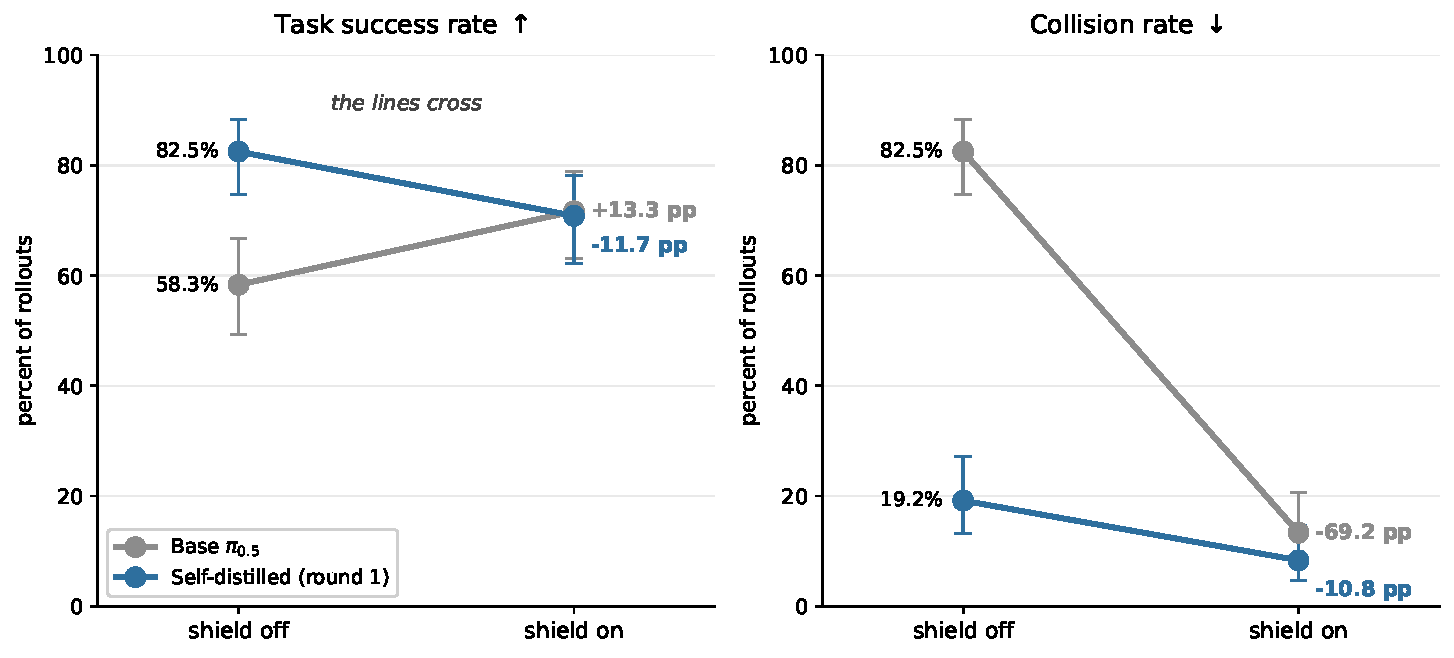
\includegraphics[width=\linewidth]{figures/fig_stacking.pdf}
  \caption[The cost of combining mechanisms]{%
  Attaching the shield raises the base policy's
    success and lowers the distilled policy's, but collisions fall in both cases.}
  \label{fig:stacking}
\end{figure}

There is a cost trade-off that comes from combining mechanisms rather than of distillation itself.
As shown in Figure~\ref{fig:stacking}, applying the shield to the distilled policy improves safety
further but reduces success by similar amounts. When the distilled policy already avoids the
obstacle, the shield's safe action projection perturbs actions that were already both safe and
competent, leading to safety-induced distribution shift. This result is congruent to what is
reported in VLSA, whose authors independently name the same effect and observe that enforcement can
drive a policy out of distribution, where it ``may behave erratically and fail to
recover''~\cite{vlsa2026}. That an approach built on runtime enforcement reports the ceiling of
runtime enforcement is the strongest available argument for internalisation, and it reaffirms the
relevance of self-distillation as an alternative route to safety that retains competence.

A second distillation round neither improved nor eroded performance, in contrast to an earlier
DAgger-style experiment in this project that degraded across rounds
(Section~\ref{sec:res:source}). One round was sufficient, and iterating was not harmful.

The trade runs both ways. Re-attaching the shield costs success but restores the online constraint
satisfaction a formal safety argument requires, and it produces the highest collision-avoidance
rate of any configuration tested --- 91.7\%, at a success rate statistically indistinguishable
from shielding the base policy. Where a safety case demands a runtime constraint, distilling first
is therefore the better starting point. That the residual is 8.3\% rather than zero is a reminder
that the guarantee is continuous-time and the implementation approximates it
(Section~\ref{sec:barrier}).

\section{Why the Corrections Transfer, and From Whom}\label{sec:disc:transfer}

Two routes to the same target were available --- move the policy toward the behaviour the shield
induces --- and they differ only in the signal used. That difference turns out to be decisive, and
for a structural reason rather than a tuning one.

A scalar reward communicates the target through one number per trajectory, leaving the policy to
infer which of several hundred actions was responsible. In a flow-matching policy the only lever
available for that inference is sampling noise, so exploration and credit assignment are the same
knob: raising it enough to distinguish good actions from bad also degrades the actions being
evaluated. Section~\ref{sec:res:channels} brackets the consequence from both sides, and no working
point exists between them. Imitation removes the inference entirely. The shield does not report
that a trajectory was unsafe; it reports what should have been done instead, at each step where it
intervened, in the space the policy emits. Credit assignment is given rather than inferred, which
is precisely what Guerrier et al.'s agent lacked: its actions were overridden while its objective
remained a scalar reward, so no gradient ever pointed toward the corrected
action~\cite{guerrier2025guardrails}.

\subsection*{What the Boundary Result Shows}

Dense per-step supervision is necessary but not sufficient. The planner's targets were equally
dense and equally corrected, and transferred nothing. What separated the two teachers was where
their demonstrations sat: at matched sampling the planner covers the states the student reaches
substantially less well (Figure~\ref{fig:state_coverage}).

The operative variable is therefore the state distribution the supervision covers, not the identity
of the teacher --- a distinction the literature supports independently. SAFE-GIL clones an MPC or
PID expert and IntervenGen replays human corrections; both teachers are foreign to the learner, and
both transfer safety, because both take care that the demonstrations sit at states the learner's
errors would produce~\cite{ciftci2025safegil,hoque2024intervengen}. Self-distillation is one route
to that coverage rather than the only one. Its practical advantage is that it needs no disturbance
model or human operator: the policy visits its own failure states unprompted.

This also sets the result against its closest conceptual neighbour. ROAD-VLA distils a corrective
signal into a VLA and argues that the teacher must remain proximal to the current
policy~\cite{wang2026roadvla}; its teacher is a perturbed copy of the student itself, and every
privileged alternative it rejects is a language template rather than a controller. Their proximity
principle therefore \emph{predicts} the planner's failure without ever testing a foreign low-level
controller. The contribution here is the measurement they anticipate rather than a disagreement
with them.

\section{What the Transfer Does Not Reach}\label{sec:disc:limits}

The transfer is uneven across the robot, and the pattern is informative rather than incidental.
Collisions were eliminated where the barrier's model of the robot is precise and the constrained
velocity is the one actually commanded, and persisted where the model is coarse and the velocity
inferred --- the arm links, which account for almost all residual collisions under the shield
(Section~\ref{sec:res:scope}). What distils is not avoidance in general but avoidance in the
channel the barrier expresses well. This is consistent with the barrier being the source of the
signal rather than a general safety prior, and it identifies the whole-body barrier as the specific
engineering change most likely to raise the ceiling.

The four alternative mechanisms failed for reasons that are legible rather than mysterious, and two
of them find independent support. The language channel produced no safety change and cost success,
which matches ROAD-VLA's account of why their own text-guided variants underperformed: a modality
gap prevents discrete text from supplying the precise grounding continuous control
requires~\cite{wang2026roadvla}. The reinforcement-learning negative reflects the poverty of a
scalar signal in the sense set out above, and the approaches that do succeed on safety-constrained
VLA training supply materially richer signals --- explicit cost constraints in a constrained
MDP~\cite{safevla}, or an action-conditioned world model that predicts the consequence of a
candidate before it is taken~\cite{safedojo} --- at a compute cost well beyond what was available
here. Best-of-$N$ selection yielded a measurement rather than a method: the near-perfect
correlation among a state's sampled candidates says that in this policy, safety is a property of
the state reached rather than of the action drawn, which is itself an argument for changing the
policy rather than for filtering its samples.

\section{Closing Summary}\label{sec:disc:summary}

This chapter interpreted the findings in relation to the four research questions of
Chapter~\ref{ch:intro}. The results support the view that a control barrier function's corrections
can be internalised into a vision-language-action policy, leaving it safer and more capable with
the shield detached --- a result that the filtering literature is structurally unable to
contradict, and that the one comparable weight-shaping study argues against~\cite{guerrier2025guardrails},
which is what makes it worth reporting. Safety and competence moved together throughout, except
where two mechanisms were stacked, an effect the primary baseline independently
documents~\cite{vlsa2026}.

The study also identified a clear boundary. Dense, in-distribution corrections transfer; equally
dense corrections from a geometry-privileged planner do not, and the variable that separates them
is state coverage rather than the teacher's identity or competence. The transfer extends only as
far as the barrier's model of the robot is faithful, and four alternative mechanisms did not
substitute for it. These findings carry implications for how safety filters are deployed and for
what remains unresolved, which the following chapter draws together.
